\subsection{Tuning behavior after ozone switches}
\label{sec:switch}

This measurement was a preliminary measurement to perform the
transition from the pure nitrogen monoxide and synthetic air setting
to unfiltered ambient air. The new challenge consists in the obvious
fact that ambient air is not \ch{NO2} free. Thus if ozone is added to
the sample air stream, one measures \ch{NO_x\, =\ NO + NO2}. In some
cases, e.\,g.\ during live vehicle measurements this is exactly what
is desired (c.\,f.~Sec.~\ref{sec:vehicle}), however, in other cases it
would be preferable to obtain the nitrogen monoxide and the nitrogen
dioxide concentrations separately. This can only be achieved
indirectly. If there is only a single cavity, \ch{NO2} and \ch{NO_x}
can be measured alternatingly by switching the ozone stream off and
on. In this case, the technical question arises of how long the
waiting time between the measurement of a \ch{NO2} and \ch{NO_x}
spectrum should be, to guarantee that all effects arising from the
ozone switch have decayed.

As Section~\ref{sec:requirements} indicates, for a tube length of
\SI{15}{\meter} the gas needs about \SI{5.3}{\second} to be completely
exchanged. Taking the cavity volume itself into account a
\SI{30}{\second} purge time should well suffice for the exchange. As
will be seen during this section, there are other unpredicted effects,
which have a far longer decay time. These have to be further
investigated before the alternating measurement mode should be used in
a productive system.

\subsubsection{Setup}
\label{sec:switch-setup}

This experiment was performed using the same setup as in
Section~\ref{sec:no} (c.\,f.\ Fig.~\ref{fig:no-setup} on
page~\pageref{fig:no-setup}). I fixed the flow of the \ch{NO}
calibration gas to $\Phi_{\ch{NO}} = \SI{0.01}{\liter\per\minute}$ and
kept all other flows as before. I set the cavity measurement script to
record 60 spectra sampled over 1000 scans each with an exposure time
of \SI{10}{\milli\second}, then to switch the ozone stream on, to
record 60 spectra with the same characteristics as before, to switch
the ozone stream off and repeat. With this setup I got a time
resolution of \SI{10}{\second}. In hindsight the sample size could
have been smaller to improve the time resolution. I performed the
measurement for both \SI{5}{\meter} and \SI{15}{\meter} reaction tube
length, due to time constraints the measurement for \SI{10}{\meter}
was shortened to only collect 30 spectra. Thus I missed some of the
decay tail in this case.

\subsubsection{Results}
\label{sec:switch-results}

Figure~\ref{fig:switch} contains the time series of the measured
\ch{NO2} concentration for a reaction tube length of $l =
\SI{15}{\meter}$. The time series for the other two tube lengths were
similar in shape and are therefore omitted here. The flanks correspond
to the switch in the ozone flow. There are severeal interesting
observations concerning this plot. First of all the increasing flanks
are very steep, which in this setting means, that the transition took
less than \SI{10}{\second}. The decreasing flanks take longer and
interestingly they do not reach \SI{0}{ppb}. This positive offset
could also be observed directly after the start of the measurement
(before any ozone had been added to the 
sample air stream). The concentration rose to a level of
\SI{1.61(2)}{ppb}. One explanation for this is, that the calibration gas is
not \ch{NO2} free. This would raise the question why I did not
measure too much \ch{NO} in Section~\ref{sec:no}, since I actually
measured \ch{NO_x}. This question has three possible answers. First, the
\ch{NO} could have converted to \ch{NO2} over time in a ratio of
one to one. This would explain why I got the right results with the official
container concentration. Alternatively, the official concentration
might not have distinguished between \ch{NO} and \ch{NO2}, but might
have only been talking about a \ch{NO_x} concentration. This second
idea could be rejected after retrieving the calibration method, which
indeed distinguished between \ch{NO} and \ch{NO2}. The last possible
explanation is that the \ch{NO2} concentration might be negligible in
comparison to the amount of \ch{NO}, thus still allowing for the good
result in the previous chapter.

Accepting for the moment that there is a background \ch{NO2} signal, I
turn towards the question, why the decreasing flanks have the slowly
falling tail. In Figure~\ref{fig:switch-pl}, there are falling flanks
for different tube lenghts and it seems that they all appear to
have a similar shape. They all seem to tend to the same equilibrium
and the decay time seems to grow with the tube length. I suspect the
reason for this long tail to be a technical one. Between the ozone
valve and the T-piece, connecting the ozone stream to the sample air
stream, there is a \SI{14}{\centi\meter} tube filled with around
\SI{200}{ppm} ozone. If this diffused into the sample line, this would
lead to further \ch{NO} conversion, although the ozone stream had
already been switched off. In order to investigate this hypothesis, I
tried to fit the decay using the following fit formula
\begin{align}
  f(t) \coloneqq c_0 + c_f \cdot\exp\left( -\frac{t}{\tau_f}\right) +
  c_s \cdot \exp\left(-\frac{t}{\tau_s}\right), \label{eq:switch-fit}
\end{align}
i.\,e.\ I suspect two overlaying decay processes. A fast one with a
decay time $\tau_f$ of less than $\SI{10}{\second}$ and a slower one
explaining the tail. Fitting this function I obtained the values
summarized in Table~\ref{tab:switch-coeff}. For the \SI{10}{\meter}
tube length fit the offset concentration had to be fixed to
\SI{1.5}{ppb}, as the measured tail was too short for it to be
determined correctly.

\begin{table}[hbtp]
  \centering
  \begin{tabular}{rSSSSSS}
    \toprule
    {$l$}& {$\tau_f$} & {$\tau_s$} & {$c_0$} & {$c_f$} & {$c_s$} & {$V_{\ch{O3}}$}\\
    {\si{\meter}}& {\si{\second}} & {\si{\second}} & {\si{ppb}} & {\si{ppb}} &
                                                      {\si{ppb}} & {\si{10\tothe{-6}\milli\liter}}\\
    \midrule
    5 & 5.95 \pm 0.13 & 141 \pm 14 & 1.48 \pm 0.03 & 16.5 \pm 0.1 
                      & 1.46 \pm 0.07 & 6.9 \pm 0.8\\
    10 & 7.04 \pm 0.15 & 146 \pm 10 & 1.5 & 19.6 \pm 0.2
                       & 2.1 \pm 0.1 & 10.2 \pm 0.1\\
    15 & 10.15 \pm 0.12 & 193 \pm 12 & 1.52 \pm 0.03 & 21.0 \pm 0.1
                        & 2.36 \pm 0.06 & 15.2 \pm 0.2\\
    \bottomrule
  \end{tabular}
  \caption{Fit coefficients for the decay function
    (Eq.~\eqref{eq:switch-fit}) after an ozone switch off. For the
    pathlength of $l= \SI{10}{\meter}$ the offset concentration was
    fixed to \SI{1.5}{ppb}. This was necessary as, due to the
    shortness of the measurement time, the tail was not long enough
    for the fit to determine the offset correctly. The last column
    contains the (partial) Volume of the ozone participating in the
    reaction to form the long tail.}
  \label{tab:switch-coeff}
\end{table}
In any case the fits underline that the decay process involves two
time scales. First, there is a rather fast one, which is well
described by the time necessary for the gas to purge the system. And a
second time scale in the order of \SIrange{2.5}{3}{\minute}. In order
to test the dead volume hypothesis, I want to use the fits to
determine the amount of ozone necessary to explain the tail. I assume
that the measured \ch{NO2} signal above the offset comes directly from
the conversion of \ch{NO} to \ch{NO2}. Looking at
Reaction~\eqref{eq:no} it becomes clear that this relation leads to a
one to one correspondence between the \ch{NO2} signal\footnote{always
  above the offset} and the amount of ozone enetering the sample air
stream. In order to determine the absolute amount, the slow falling
part of the fit function has to be integrated and the constant flow of
$\Phi = \SI{2}{\liter\per\minute}$ has to be used to convert the
result to the (partial) volume of ozone, i.\,e.
\begin{align*}
  V_{\ch{O3}} \coloneqq  c_s \cdot \tau_s \cdot \Phi.
\end{align*}
The result of this computation can be found in
Table~\ref{tab:switch-coeff}, too. A first observation is the clear
pathlength dependence. This is already an indicator against my
hypothesis, as the dead volume is constant. Nevertheless, computing
the ozone volume in the tube leads to
\begin{align*}
  V_{\text{tube}} \approx \SI{3.52e-4}{\milli\liter}.
\end{align*}
This is even more evidence that the dead volume cannot be the sole
explanation. The total ozone volume is about two orders of magnitude
too large. Even if I take into account that not the whole tube volume
contributes to the reaction (as the ozone enters the sample air stream
via diffusion), I still have to explain the pathlength
dependence. Especially as it seems that the relation is highly linear,
one might suspect the reason to lie in the adsorption capacity of the
teflon tubes. This capacity would have to be researched more deeply
than I can provide at the current time, however, if the adsorption
plays an important role in the decay behavior of the system, this
would lead to a further important restriction concerning the
measurement method. The alternating measurement mode would become
impractical to use, as the purge time would have to be in the order of
magnitude of multiple minutes. This is inacceptable for volatile
environments as for example urban areas.

\begin{figure}[htbp]
  \centering
  % GNUPLOT: LaTeX picture with Postscript
\begingroup
  \makeatletter
  \providecommand\color[2][]{%
    \GenericError{(gnuplot) \space\space\space\@spaces}{%
      Package color not loaded in conjunction with
      terminal option `colourtext'%
    }{See the gnuplot documentation for explanation.%
    }{Either use 'blacktext' in gnuplot or load the package
      color.sty in LaTeX.}%
    \renewcommand\color[2][]{}%
  }%
  \providecommand\includegraphics[2][]{%
    \GenericError{(gnuplot) \space\space\space\@spaces}{%
      Package graphicx or graphics not loaded%
    }{See the gnuplot documentation for explanation.%
    }{The gnuplot epslatex terminal needs graphicx.sty or graphics.sty.}%
    \renewcommand\includegraphics[2][]{}%
  }%
  \providecommand\rotatebox[2]{#2}%
  \@ifundefined{ifGPcolor}{%
    \newif\ifGPcolor
    \GPcolorfalse
  }{}%
  \@ifundefined{ifGPblacktext}{%
    \newif\ifGPblacktext
    \GPblacktexttrue
  }{}%
  % define a \g@addto@macro without @ in the name:
  \let\gplgaddtomacro\g@addto@macro
  % define empty templates for all commands taking text:
  \gdef\gplbacktext{}%
  \gdef\gplfronttext{}%
  \makeatother
  \ifGPblacktext
    % no textcolor at all
    \def\colorrgb#1{}%
    \def\colorgray#1{}%
  \else
    % gray or color?
    \ifGPcolor
      \def\colorrgb#1{\color[rgb]{#1}}%
      \def\colorgray#1{\color[gray]{#1}}%
      \expandafter\def\csname LTw\endcsname{\color{white}}%
      \expandafter\def\csname LTb\endcsname{\color{black}}%
      \expandafter\def\csname LTa\endcsname{\color{black}}%
      \expandafter\def\csname LT0\endcsname{\color[rgb]{1,0,0}}%
      \expandafter\def\csname LT1\endcsname{\color[rgb]{0,1,0}}%
      \expandafter\def\csname LT2\endcsname{\color[rgb]{0,0,1}}%
      \expandafter\def\csname LT3\endcsname{\color[rgb]{1,0,1}}%
      \expandafter\def\csname LT4\endcsname{\color[rgb]{0,1,1}}%
      \expandafter\def\csname LT5\endcsname{\color[rgb]{1,1,0}}%
      \expandafter\def\csname LT6\endcsname{\color[rgb]{0,0,0}}%
      \expandafter\def\csname LT7\endcsname{\color[rgb]{1,0.3,0}}%
      \expandafter\def\csname LT8\endcsname{\color[rgb]{0.5,0.5,0.5}}%
    \else
      % gray
      \def\colorrgb#1{\color{black}}%
      \def\colorgray#1{\color[gray]{#1}}%
      \expandafter\def\csname LTw\endcsname{\color{white}}%
      \expandafter\def\csname LTb\endcsname{\color{black}}%
      \expandafter\def\csname LTa\endcsname{\color{black}}%
      \expandafter\def\csname LT0\endcsname{\color{black}}%
      \expandafter\def\csname LT1\endcsname{\color{black}}%
      \expandafter\def\csname LT2\endcsname{\color{black}}%
      \expandafter\def\csname LT3\endcsname{\color{black}}%
      \expandafter\def\csname LT4\endcsname{\color{black}}%
      \expandafter\def\csname LT5\endcsname{\color{black}}%
      \expandafter\def\csname LT6\endcsname{\color{black}}%
      \expandafter\def\csname LT7\endcsname{\color{black}}%
      \expandafter\def\csname LT8\endcsname{\color{black}}%
    \fi
  \fi
    \setlength{\unitlength}{0.0500bp}%
    \ifx\gptboxheight\undefined%
      \newlength{\gptboxheight}%
      \newlength{\gptboxwidth}%
      \newsavebox{\gptboxtext}%
    \fi%
    \setlength{\fboxrule}{0.5pt}%
    \setlength{\fboxsep}{1pt}%
\begin{picture}(7200.00,5040.00)%
    \gplgaddtomacro\gplbacktext{%
      \csname LTb\endcsname%
      \put(682,704){\makebox(0,0)[r]{\strut{}$0$}}%
      \put(682,1383){\makebox(0,0)[r]{\strut{}$5$}}%
      \put(682,2061){\makebox(0,0)[r]{\strut{}$10$}}%
      \put(682,2740){\makebox(0,0)[r]{\strut{}$15$}}%
      \put(682,3418){\makebox(0,0)[r]{\strut{}$20$}}%
      \put(682,4097){\makebox(0,0)[r]{\strut{}$25$}}%
      \put(682,4775){\makebox(0,0)[r]{\strut{}$30$}}%
      \put(814,484){\makebox(0,0){\strut{}$0$}}%
      \put(1563,484){\makebox(0,0){\strut{}$500$}}%
      \put(2311,484){\makebox(0,0){\strut{}$1000$}}%
      \put(3060,484){\makebox(0,0){\strut{}$1500$}}%
      \put(3809,484){\makebox(0,0){\strut{}$2000$}}%
      \put(4557,484){\makebox(0,0){\strut{}$2500$}}%
      \put(5306,484){\makebox(0,0){\strut{}$3000$}}%
      \put(6054,484){\makebox(0,0){\strut{}$3500$}}%
      \put(6803,484){\makebox(0,0){\strut{}$4000$}}%
    }%
    \gplgaddtomacro\gplfronttext{%
      \csname LTb\endcsname%
      \put(176,2739){\rotatebox{-270}{\makebox(0,0){\strut{}Concentration [ppb]}}}%
      \put(3808,154){\makebox(0,0){\strut{}Time [s]}}%
    }%
    \gplbacktext
    \put(0,0){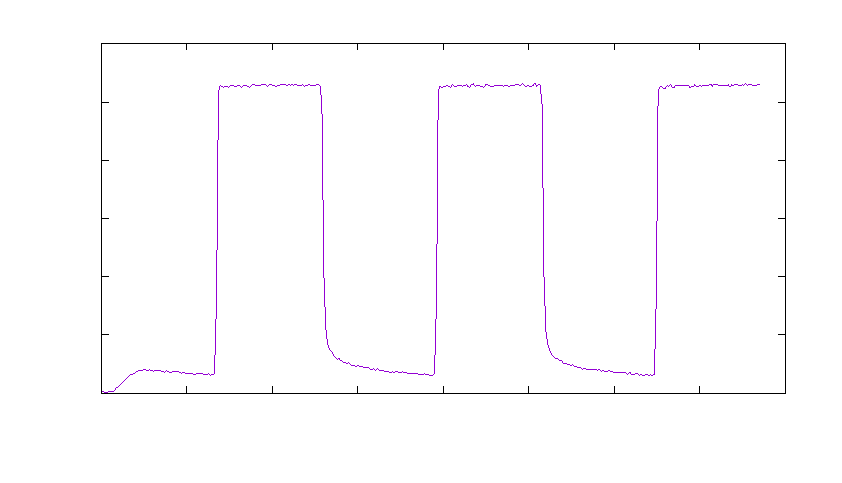
\includegraphics{../images/20160223_15_equil_fixI0_ts}}%
    \gplfronttext
  \end{picture}%
\endgroup

  \caption{Time series of the measured \ch{NO2} concentration while
    switching the ozone stream on and off.}
  \label{fig:switch}
\end{figure}
\begin{figure}[htbp]
  \centering
  % GNUPLOT: LaTeX picture with Postscript
\begingroup
  \makeatletter
  \providecommand\color[2][]{%
    \GenericError{(gnuplot) \space\space\space\@spaces}{%
      Package color not loaded in conjunction with
      terminal option `colourtext'%
    }{See the gnuplot documentation for explanation.%
    }{Either use 'blacktext' in gnuplot or load the package
      color.sty in LaTeX.}%
    \renewcommand\color[2][]{}%
  }%
  \providecommand\includegraphics[2][]{%
    \GenericError{(gnuplot) \space\space\space\@spaces}{%
      Package graphicx or graphics not loaded%
    }{See the gnuplot documentation for explanation.%
    }{The gnuplot epslatex terminal needs graphicx.sty or graphics.sty.}%
    \renewcommand\includegraphics[2][]{}%
  }%
  \providecommand\rotatebox[2]{#2}%
  \@ifundefined{ifGPcolor}{%
    \newif\ifGPcolor
    \GPcolorfalse
  }{}%
  \@ifundefined{ifGPblacktext}{%
    \newif\ifGPblacktext
    \GPblacktexttrue
  }{}%
  % define a \g@addto@macro without @ in the name:
  \let\gplgaddtomacro\g@addto@macro
  % define empty templates for all commands taking text:
  \gdef\gplbacktext{}%
  \gdef\gplfronttext{}%
  \makeatother
  \ifGPblacktext
    % no textcolor at all
    \def\colorrgb#1{}%
    \def\colorgray#1{}%
  \else
    % gray or color?
    \ifGPcolor
      \def\colorrgb#1{\color[rgb]{#1}}%
      \def\colorgray#1{\color[gray]{#1}}%
      \expandafter\def\csname LTw\endcsname{\color{white}}%
      \expandafter\def\csname LTb\endcsname{\color{black}}%
      \expandafter\def\csname LTa\endcsname{\color{black}}%
      \expandafter\def\csname LT0\endcsname{\color[rgb]{1,0,0}}%
      \expandafter\def\csname LT1\endcsname{\color[rgb]{0,1,0}}%
      \expandafter\def\csname LT2\endcsname{\color[rgb]{0,0,1}}%
      \expandafter\def\csname LT3\endcsname{\color[rgb]{1,0,1}}%
      \expandafter\def\csname LT4\endcsname{\color[rgb]{0,1,1}}%
      \expandafter\def\csname LT5\endcsname{\color[rgb]{1,1,0}}%
      \expandafter\def\csname LT6\endcsname{\color[rgb]{0,0,0}}%
      \expandafter\def\csname LT7\endcsname{\color[rgb]{1,0.3,0}}%
      \expandafter\def\csname LT8\endcsname{\color[rgb]{0.5,0.5,0.5}}%
    \else
      % gray
      \def\colorrgb#1{\color{black}}%
      \def\colorgray#1{\color[gray]{#1}}%
      \expandafter\def\csname LTw\endcsname{\color{white}}%
      \expandafter\def\csname LTb\endcsname{\color{black}}%
      \expandafter\def\csname LTa\endcsname{\color{black}}%
      \expandafter\def\csname LT0\endcsname{\color{black}}%
      \expandafter\def\csname LT1\endcsname{\color{black}}%
      \expandafter\def\csname LT2\endcsname{\color{black}}%
      \expandafter\def\csname LT3\endcsname{\color{black}}%
      \expandafter\def\csname LT4\endcsname{\color{black}}%
      \expandafter\def\csname LT5\endcsname{\color{black}}%
      \expandafter\def\csname LT6\endcsname{\color{black}}%
      \expandafter\def\csname LT7\endcsname{\color{black}}%
      \expandafter\def\csname LT8\endcsname{\color{black}}%
    \fi
  \fi
    \setlength{\unitlength}{0.0500bp}%
    \ifx\gptboxheight\undefined%
      \newlength{\gptboxheight}%
      \newlength{\gptboxwidth}%
      \newsavebox{\gptboxtext}%
    \fi%
    \setlength{\fboxrule}{0.5pt}%
    \setlength{\fboxsep}{1pt}%
\begin{picture}(7200.00,5040.00)%
    \gplgaddtomacro\gplbacktext{%
      \csname LTb\endcsname%
      \put(682,704){\makebox(0,0)[r]{\strut{}$0$}}%
      \put(682,1518){\makebox(0,0)[r]{\strut{}$5$}}%
      \put(682,2332){\makebox(0,0)[r]{\strut{}$10$}}%
      \put(682,3147){\makebox(0,0)[r]{\strut{}$15$}}%
      \put(682,3961){\makebox(0,0)[r]{\strut{}$20$}}%
      \put(682,4775){\makebox(0,0)[r]{\strut{}$25$}}%
      \put(814,484){\makebox(0,0){\strut{}$0$}}%
      \put(1670,484){\makebox(0,0){\strut{}$100$}}%
      \put(2525,484){\makebox(0,0){\strut{}$200$}}%
      \put(3381,484){\makebox(0,0){\strut{}$300$}}%
      \put(4236,484){\makebox(0,0){\strut{}$400$}}%
      \put(5092,484){\makebox(0,0){\strut{}$500$}}%
      \put(5947,484){\makebox(0,0){\strut{}$600$}}%
      \put(6803,484){\makebox(0,0){\strut{}$700$}}%
    }%
    \gplgaddtomacro\gplfronttext{%
      \csname LTb\endcsname%
      \put(176,2739){\rotatebox{-270}{\makebox(0,0){\strut{}Concentration [ppb]}}}%
      \put(3808,154){\makebox(0,0){\strut{}Time [s]}}%
      \csname LTb\endcsname%
      \put(5816,4602){\makebox(0,0)[r]{\strut{}$\SI{05}{\meter}$}}%
      \csname LTb\endcsname%
      \put(5816,4382){\makebox(0,0)[r]{\strut{}$\SI{10}{\meter}$}}%
      \csname LTb\endcsname%
      \put(5816,4162){\makebox(0,0)[r]{\strut{}$\SI{15}{\meter}$}}%
    }%
    \gplbacktext
    \put(0,0){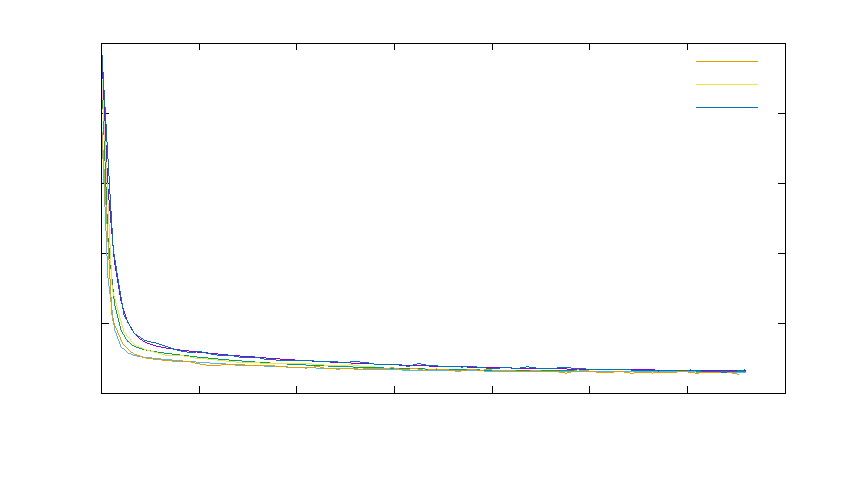
\includegraphics{../images/20160223_equil_fixI0_fall_fit}}%
    \gplfronttext
  \end{picture}%
\endgroup

  \caption{The behavior of the falling flanks depending on the
    reaction pathlength}
  \label{fig:switch-pl}
\end{figure}

If the alternating mode is to be used anyways, one would have to
compensate for the long tail. For the laboratory conditions, used in
this experiment, the supply of \ch{NO} was constant, which means that
the behavior of the falling flank was solely determined by the
changing ozone concentration. Assuming that the decay always follows
Equation~\eqref{eq:switch-fit} with the coefficients given in
Table~\ref{tab:switch-coeff}, the average additional \ch{NO2} signal
due to the flank can be computed by

\begin{align}
  \bar c_s = \frac{c_s}{\Delta t} \int_{t_0}^{t_1}
  \exp\left(-\frac{t}{\tau_s}\right)\d[t] \approx \SI{1.55(8)}{ppb},\label{eq:offset}
\end{align}
with $t_0 = \SI{30}{\second}$, $t_1 = \SI{60}{\second}$,
$\Delta t = t_1 - t_0$, where I already specialized to the later used
setup of $l = \SI{10}{\meter}$. I propose now to correct the measured
\ch{NO2} values by this offset. For this procedure to work, the decay
form would need to be mainly \ch{NO} independent. This assumption
might be true, as the bottle neck in Reaction~\eqref{eq:no} should be
the vanishing ozone. However, to be sure, I would suggest to perform
further decay experiments at multiple \ch{NO} levels. This would lead
to the further advantage, that possible existing \ch{NO} dependencies
could probably be extrapolated. This in turn would lead to a \ch{NO_x}
dependent offset correction in the evaluation procedure.  In the
following I tested the limits of this rather crude approximation. The
results can be found in the next section.

%%% Local Variables:
%%% mode: latex
%%% TeX-master: "../Bachelor"
%%% End:
